\documentclass[a4paper]{oblivoir}

\title{쟤료공학개론 과제6}
\author{2018-12432, Electrical and Computer Engineering department, ParkJeonghyun}
\date{11/12/2023}

\newcommand{\be}{\begin{equation}}
\newcommand{\ee}{\end{equation}}

\usepackage{fapapersize}
\usepackage{amsmath}
\usepackage{MnSymbol}
\usepackage{wasysym}
\usepackage{graphicx}
\usepackage{caption}
\usepackage{subfig}
\usepackage{hyperref}
\usepackage{cite}
\usepackage{dtk-logos}
\usepackage{physics}
\usepackage{tikz}
\usetikzlibrary{decorations.markings, positioning}
\usepackage{dtk-logos}
\usepackage{fancyvrb}
\usepackage{array} 
\usepackage{chemformula}

\usefapapersize{ 210mm, 297mm, 15mm, 15mm, 15mm, 15mm}
\DeclareGraphicsExtensions{.pdf, .png, .jpg}

\renewcommand{\figurename}{Figure}

\begin{document}

\maketitle
\section{Problem 1}
\begin{align}
	\sigma_{m} &= 2\sigma_{0}\left( \frac{a}{\rho_{t}} \right)^{1/2}\\
	&= 2\times 1035 \times 10^{6}\left( \frac{0.5}{5\times10^{-3}} \right)^{1/2} Pa\\
	&= 20.7 GPa
\end{align}

\section{Problem 2}
Fracture toughness는 아래식을 만족한다.
\begin{align}
	K_{c} &= Y\sigma\sqrt{\pi a}
\end{align}
따라서 Y는 아래와 같다.
\begin{align}
	Y &= \frac{K_{c}}{\sigma\sqrt{\pi a}}\\
	&= \frac{26.0\times 10^{6}}{112 \times 10^{6}\times\sqrt{\pi \times 8.6\times10^{-3}}} \\
	&=1.4123
\end{align}
따라서 6.0mm의 crack length에 대해서 stree level은 아래와 같다.
\begin{align}
	\sigma &= \frac{K_{c}}{\sqrt{\pi a}Y}\\
	&= \frac{26.0\times 10^{6}}{\sqrt{\pi \times 6.0\times10^{-3}}\times1.4123}Pa\\
	&= 134 MPa
\end{align}

\section{Problem 3}
\subsection{a}
그래프는 Fig.\ref{fig:pro3}와 같다.
\begin{figure}[htbp]
	\begin{centering}
	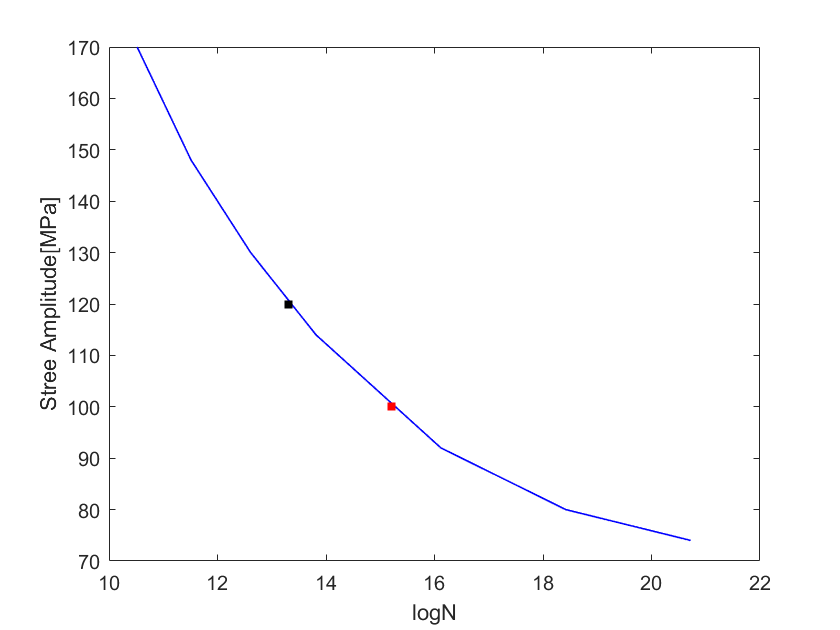
\includegraphics[width = 0.75\linewidth]{pro3.png}% Here is how to import EPS art
	\caption{\label{fig:pro3} S-N graph}
	\end{centering}
\end{figure}

\subsection{b}
$N = 4\times10^{6}$일 때 약 100MPa이다.(Fig.\ref{fig:pro3} 빨간점)

\subsection{b}
120MPa일 때 약 $N = 6\times10^{5}$이다.(Fig.\ref{fig:pro3} 검은점)

\end{document}